\documentclass[11pt]{article}

\usepackage[margin=0.85in]{geometry}
\usepackage{amsmath}
\usepackage{booktabs}
\usepackage{graphicx}
\usepackage[hidelinks]{hyperref}
\usepackage{xcolor}

\definecolor{sommerfeld}{RGB}{213,94,0}
\definecolor{cpbc}{RGB}{0,114,178}
\newcommand{\hash}[2]{\texttt{#1}\allowbreak\texttt{#2}}

\title{Thin-z TDE Outer-Boundary Comparison\\
\large Extrapolated Sommerfeld versus Zero-Rate Characteristic CPBC}
\author{AthenaK Z4c validation}
\date{July 30, 2026}

\begin{document}
\maketitle

\begin{abstract}
We compare two no-sponge tidal-disruption-event evolutions with identical
initial data, mesh, executable, MPI decomposition and placement policy, and
fourth-order boundary extrapolation.  The only intentional physical or
numerical boundary difference is the outer-boundary right-hand side:
extrapolated Sommerfeld or the archived zero-rate characteristic
constraint-preserving boundary condition (CPBC).
Sommerfeld develops a lower-$z$-localized instability at $t/M\simeq 7$ and
becomes nonfinite at $t/M=7.2$.  The CPBC evolution remains finite through
$t/M=30$, with decreasing global constraint norms and a bounded close-face
Hamiltonian maximum.  Its orbital-plane density slices retain a coherent,
nearly circular stellar core throughout the run.  Thus the archived
zero-rate CPBC cures the observed instability in this configuration.  This
result does not validate the newer experimental tangential-principal
implementation, and a matched far-boundary reference is still required for
formal reflection, density, and trajectory acceptance gates.
\end{abstract}

\section{Question and answer}

For the tested thin-$z$ TDE configuration, the answer is yes: the archived
zero-rate CPBC prevents the instability exhibited by extrapolated
Sommerfeld.  The conclusion is empirical and configuration-specific.  It is
supported by a byte-identical executable comparison and by survival for more
than three nominal fastest-gauge round trips.

\section{Matched setup}

Both evolutions used executable SHA-256
\begin{center}
\hash{cd7cefef042ff075e85688dd3ec08dca}
{243df479d50b91e0439dd8a20da46478}.
\end{center}
The domain and numerical settings were:
\begin{center}
\begin{tabular}{ll}
\toprule
Quantity & Value \\
\midrule
Domain & $x\in[-48,72]M$, $y\in[-48,48]M$, $z\in[-6,42]M$ \\
Initial star center & approximately $(40,0,0)M$ \\
Root spacing & $0.75M$ \\
Target time & $30M$ \\
Close physical face & lower $z$ \\
Boundary extrapolation & order 4 \\
Outer sponge & explicitly disabled \\
Resources & 32 Aurora nodes, 12 MPI ranks per node \\
\bottomrule
\end{tabular}
\end{center}

The Sommerfeld reproducer was job \texttt{8718377}.  The CPBC evolution used
fresh segment \texttt{8718576} and restart segments \texttt{8718778},
\texttt{8718933}, and \texttt{8719210}.  Every CPBC segment exited with
status zero.  Each restart generation contained exactly 384 nonempty
rank-local members.

\section{Evolution outcome}

\begin{figure}[htbp]
\centering
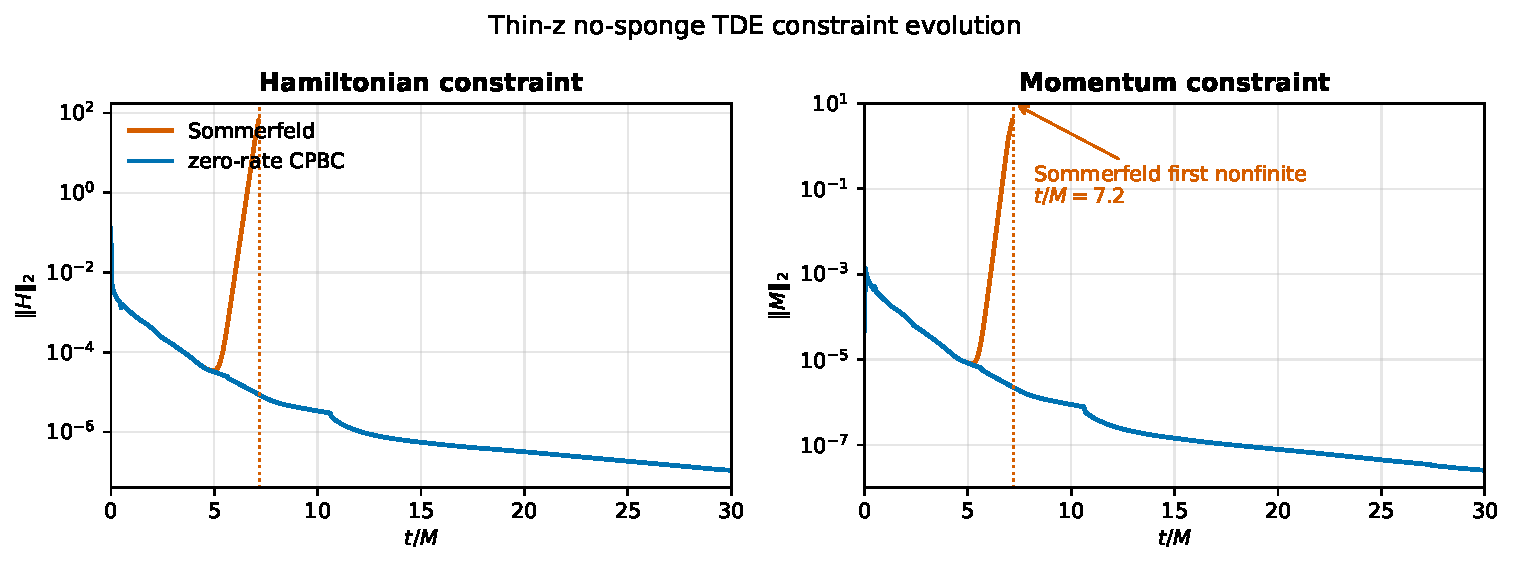
\includegraphics[width=\textwidth]{figures/tde_boundary_constraint_histories.pdf}
\caption{Global Hamiltonian and momentum constraint histories.  The two
curves agree before the causal return.  Sommerfeld then grows catastrophically
and becomes nonfinite at $t/M=7.2$, while CPBC continues to $t/M=30$ with
decreasing norms.}
\label{fig:constraints}
\end{figure}

The first material Sommerfeld growth appears at the lower-$z$ face:
\[
\begin{array}{c|c|c}
t/M & \max |H| & (x,y,z)/M\\
\hline
7.00313 & 31.8178 & (-0.0703,0.4453,-5.9766)\\
7.05234 & 39.3038 & (-0.0703,0.4453,-5.9766)\\
7.10156 & 44.4944 & (2.1797,-0.0703,-5.9766)\\
7.15078 & 69.0354 & (2.0391,0.0703,-5.9766)
\end{array}
\]
The first nonfinite history row is at $t/M=7.2$.  Shortly afterward the
stellar density tracker falls to the atmosphere floor.

At the matched finite history sample $t/M=7.1015625$, the global comparison
is:
\begin{center}
\begin{tabular}{lrrr}
\toprule
Diagnostic & Sommerfeld & CPBC & Sommerfeld/CPBC \\
\midrule
$\|H\|_2$ & $4.76992\times10^{1}$ & $9.00521\times10^{-6}$ &
$5.297\times10^{6}$ \\
$\|M\|_2$ & $3.13449$ & $2.37331\times10^{-6}$ &
$1.321\times10^{6}$ \\
$\|\Theta\|$ & $4.32375\times10^{-5}$ & $1.30143\times10^{-8}$ &
$3.322\times10^{3}$ \\
$\max|\Theta|$ & $3.85857\times10^{-2}$ & $1.80522\times10^{-5}$ &
$2.137\times10^{3}$ \\
$\max|\delta\alpha|$ & $1.08070\times10^{-2}$ & $9.48888\times10^{-6}$ &
$1.139\times10^{3}$ \\
$\max|\delta\beta^i|$ & $3.24569\times10^{-4}$ & $3.58307\times10^{-6}$ &
$9.058\times10^{1}$ \\
$\max|\delta\widetilde{\Gamma}^{i}|$ & $3.20782\times10^{-3}$ &
$2.15356\times10^{-5}$ & $1.490\times10^{2}$ \\
\bottomrule
\end{tabular}
\end{center}

\begin{figure}[htbp]
\centering
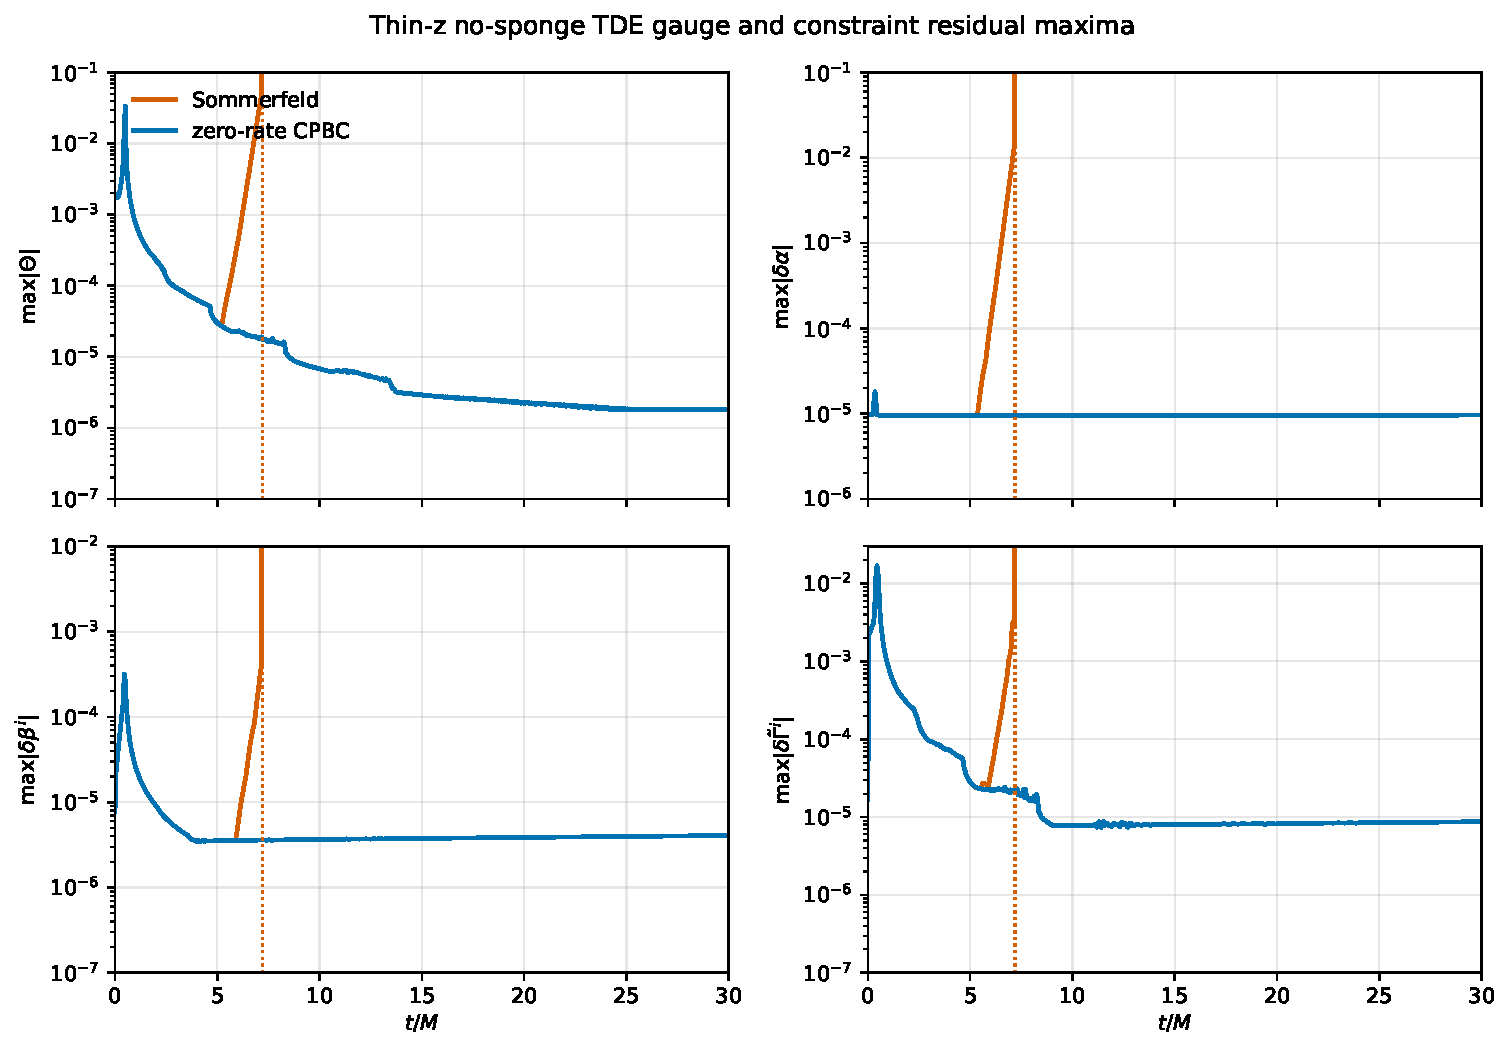
\includegraphics[width=\textwidth]{figures/tde_boundary_residual_histories.pdf}
\caption{Gauge and constraint residual maxima.  Fixed vertical ranges retain
the pre-failure CPBC baseline and the Sommerfeld onset; catastrophic
Sommerfeld values beyond the displayed range clip at the upper axis.}
\label{fig:residuals}
\end{figure}

\begin{figure}[htbp]
\centering
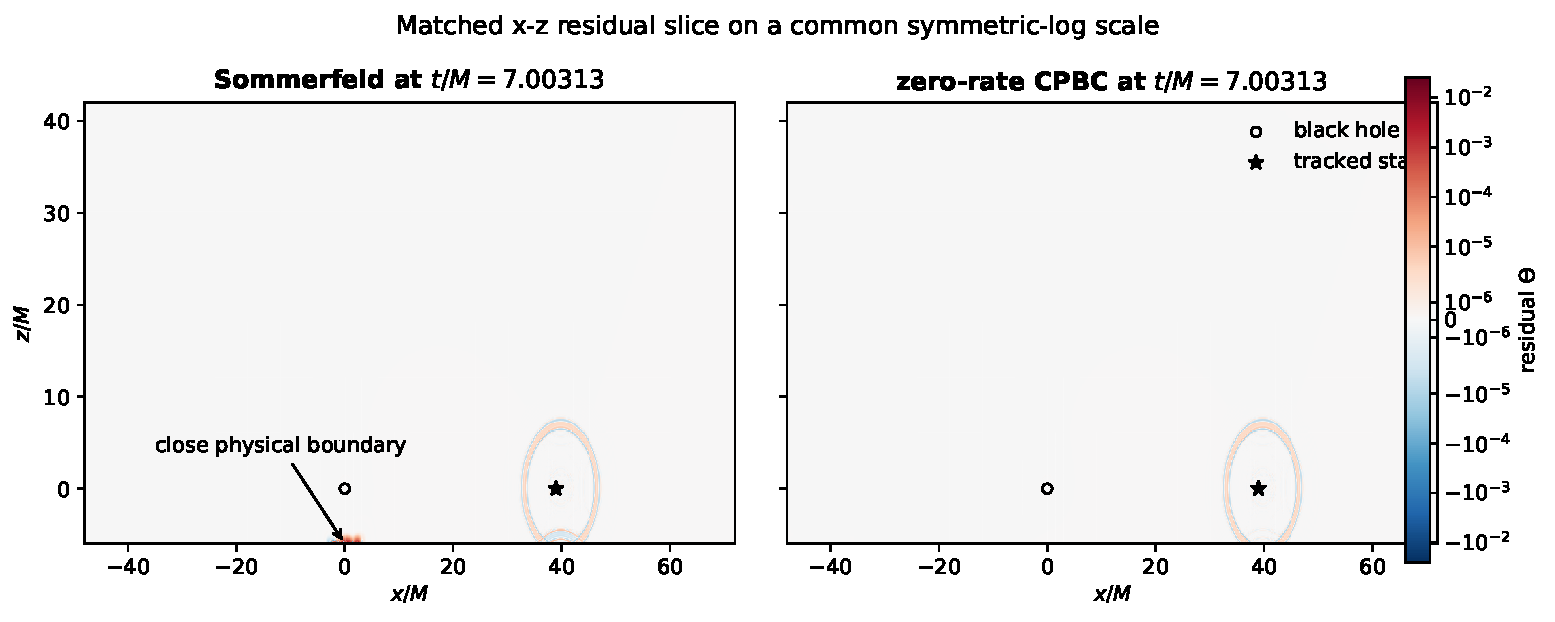
\includegraphics[width=\textwidth]{figures/tde_boundary_theta_slice_t7.pdf}
\caption{Matched $x$-$z$ residual $\Theta$ slices at $t/M=7.00313$ on a
common symmetric-logarithmic scale.  Sommerfeld has already developed a
strong localized feature at the close lower-$z$ boundary near the black
hole.  The CPBC slice remains bounded.}
\label{fig:slice}
\end{figure}

\clearpage
\subsection{Orbital-plane stellar morphology}

The available fluid slices resolve the $x$--$y$ orbital plane.  We measured
all 61 CPBC density outputs rather than inferring shape from
$\rho_{\max}$ alone.  At each time, the dense-core region is defined by
$\rho\geq\rho_{\max}/2$; its area gives
$R_{1/2}=\sqrt{A_{1/2}/\pi}$, and a density-weighted covariance gives the
principal-axis ratio $a/b$.  A peak-centered, peak-normalized density map
provides a separate shape-$L_2$ diagnostic.

\begin{center}
\begin{tabular}{lccc}
\toprule
Diagnostic & Initial & Range through $30M$ & Final \\
\midrule
$\rho_{\max}$ & $1.22674\times10^{-4}$
  & $-0.10\%$ to $+4.89\%$ & $1.28672\times10^{-4}$ \\
$R_{1/2}/M$ & $0.08363$
  & $-0.63\%$ to $+1.24\%$ & $0.08311$ \\
$a/b$ & $1.0065$ & $1.0005$ to $1.0748$ & $1.0282$ \\
Centered shape $L_2$ & 0 & 0 to $0.0738$ & $0.0442$ \\
\bottomrule
\end{tabular}
\end{center}

\begin{figure}[htbp]
\centering
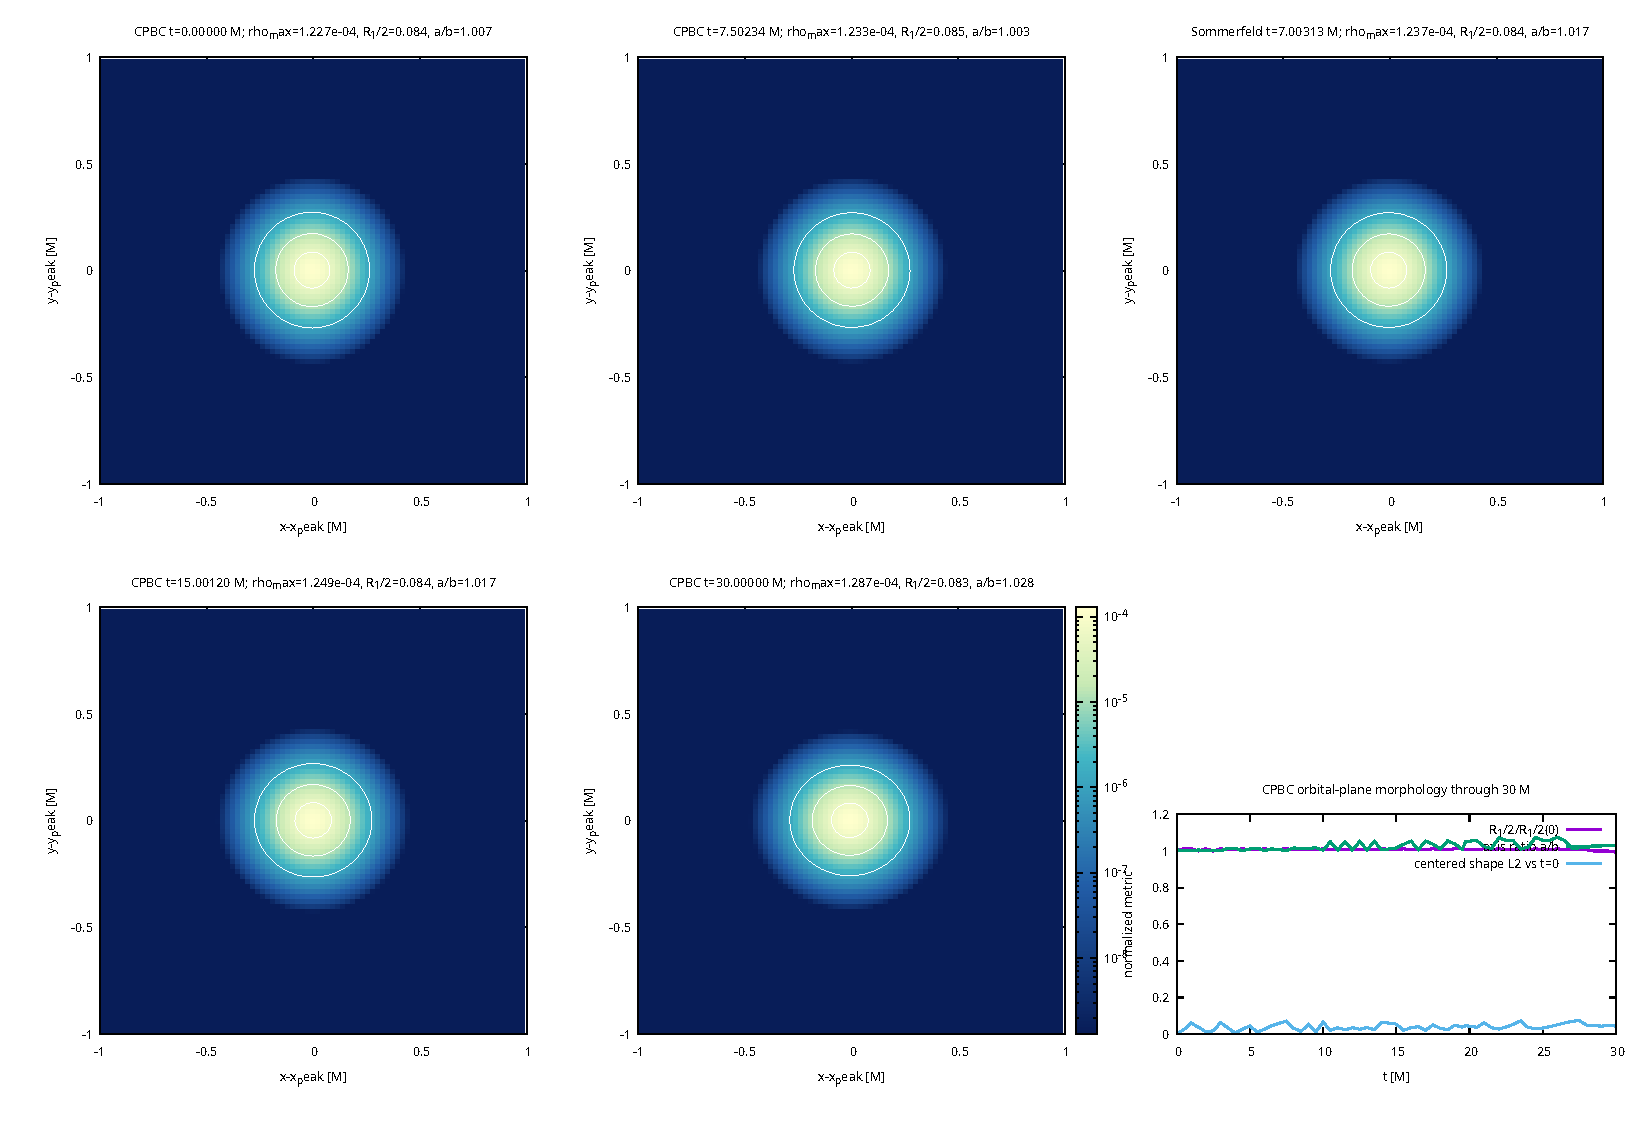
\includegraphics[width=\textwidth]
  {figures/tde_stellar_morphology_cpbc_vs_sommerfeld.pdf}
\caption{Peak-centered orbital-plane density with a common absolute
logarithmic color scale.  White contours mark 50, 10, and 1 percent of each
panel's peak.  The lower-right panel summarizes all 61 CPBC outputs.
Sommerfeld is shown at $t/M=7.00313$, when the boundary failure is already
material but the star remains physical.  No CPBC density slice was stored at
that exact time; the nearest displayed CPBC slice is $t/M=7.50234$, offset
by $0.49921M$.}
\label{fig:morphology}
\end{figure}

The Sommerfeld slice was deliberately chosen before its density becomes
floor-dominated: it has
$\rho_{\max}=1.23677\times10^{-4}$ and close-face
$\max|H|=31.8178$.  Its $R_{1/2}=0.08415M$ and $a/b=1.0169$ remain
stellar.  The nearest CPBC slice has $R_{1/2}=0.08467M$ and
$a/b=1.0029$; their centered normalized density maps differ by 0.0677,
with the stated $0.49921M$ time offset.

These measurements support a positive, qualified answer to the shape
question: the CPBC run preserves a single coherent and resolved
orbital-plane stellar core through $30M$, with at most 7.5 percent
ellipticity in this diagnostic.  They do not establish the unobserved
vertical profile or full three-dimensional shape, nor do they replace the
still-open far-reference density and trajectory gates.

\section{CPBC state at the target time}

The CPBC case reaches $t/M=30$ with no nonfinite, bad-metric, MPI, SYCL,
GPU, or restart error.  Its final diagnostics are:
\begin{center}
\begin{tabular}{lr}
\toprule
Diagnostic & Value at $t/M=30$ \\
\midrule
$\|H\|_2$ & $1.09007\times10^{-7}$ \\
$\|M\|_2$ & $2.56218\times10^{-8}$ \\
Close-face $\max|H|$ & $1.20496\times10^{-4}$ \\
$\rho_{\max}$ & $1.28672\times10^{-4}$ \\
Tracked star position & $(35.3731,-0.00586,-0.00586)M$ \\
Bad-metric count & 0 \\
\bottomrule
\end{tabular}
\end{center}

An independent late-time projection over 13 slices in $t/M\in[27,30]$
reports all ten incoming characteristic families:
\begin{center}
\begin{tabular}{lr@{\qquad}lr}
\toprule
Family & Maximum RMS & Family & Maximum RMS \\
\midrule
Lapse & $3.22520\times10^{-6}$ &
Longitudinal shift & $3.45682\times10^{-6}$ \\
Transverse shift 1 & $1.83089\times10^{-6}$ &
Transverse shift 2 & $8.37305\times10^{-9}$ \\
Scalar constraint $\Theta$ & $6.41182\times10^{-6}$ &
Scalar constraint $Z$ & $1.07866\times10^{-6}$ \\
Transverse constraint 1 & $1.69201\times10^{-6}$ &
Transverse constraint 2 & $1.08745\times10^{-8}$ \\
TT plus & $1.34214\times10^{-6}$ &
TT cross & $8.72326\times10^{-8}$ \\
\bottomrule
\end{tabular}
\end{center}
All remain finite and $O(10^{-6})$ or smaller over
$27\leq t/M\leq30$.  Incoming and outgoing rows are reconstructed from the
full evolved conformal metric and independently transcribed characteristic
formulae; boundary-enforcement diagnostics are not used as reflection
measurements.

\section{Analysis safeguards}

Restarted outputs duplicate the state at each segment boundary.  The reader
finds duplicate slice times at $6.50039M$, $14.0027M$, and $19.7508M$.
Each pair has identical mesh layout and exactly zero field difference,
although binary header metadata differs.  The analysis collapses only
field-identical duplicates and rejects conflicting duplicates.

The lower-face Sommerfeld metric becomes sufficiently distorted that the
face-normal frame develops an out-of-$x$-$z$-plane component of
$1.00845\times10^{-3}$.  Because an $x$-$z$ slice cannot supply the missing
$y$ derivative, the post-failure all-ten face projection is rejected rather
than evaluated with a coordinate-aligned approximation.  Raw
coordinate-bearing extrema still localize the instability at the first
lower-$z$ cell layer.

\section{Scope and limitations}

This report validates the archived zero-rate executable in the selected TDE
comparison.  The source branch also contains a newer experimental
tangential-principal target.  That newer implementation was not used in
these TDE jobs and must not inherit this validation claim.

The existing far-boundary reference has different thin-$z$ geometry,
different residual-slice coverage, and no executable parity through
$t/M=30$.  Therefore this comparison does not yet measure a
far-reference-subtracted returning characteristic signal.  The formal
tenfold gauge/constraint reflection gate, the per-family 10 percent
non-regression gate, the one percent density gate, and the
$0.1R_{\star}$ trajectory gate remain open.  A matched far-boundary run
with $x$-$z$ residual output is required for those claims.

\section{Reproducibility}

The figures are regenerated by:
\begin{verbatim}
python3 analysis/z4c_characteristic/plot_tde_boundary_comparison.py \
  --sommerfeld <sommerfeld-run> \
  --cpbc <cpbc-run> \
  --output-dir docs/z4c/figures --formats pdf
python3 analysis/z4c_characteristic/plot_tde_stellar_morphology.py \
  --sommerfeld-run <sommerfeld-run> \
  --cpbc-run <cpbc-run> \
  --output docs/z4c/figures/tde_stellar_morphology_cpbc_vs_sommerfeld.pdf \
  --metrics-csv docs/z4c/figures/tde_stellar_morphology_metrics.csv
\end{verbatim}
The late CPBC projection log has SHA-256
\begin{center}
\hash{24ddd2d0cdba5fe7e975d785e8c4d2a7}
{ccd7ae6b0f1644e2dd1c5c4298105856}.
\end{center}
The causal Sommerfeld and CPBC projection logs have SHA-256 values
\begin{center}
\hash{380c58c27faf947ff36d0f994ac18d503}
{d245c1dab7bd2e380f477c29f99af49}\\
\hash{f04b710b4fcf1bc466b680b8a6d1204}
{b7b140ee5d533f1558548b203e14ae71d}
\end{center}
for Sommerfeld and CPBC, respectively.

\section{Conclusion}

In the matched no-sponge thin-$z$ TDE experiment, extrapolated Sommerfeld
causes a causally timed, lower-boundary-localized instability and becomes
nonfinite.  The archived zero-rate CPBC removes that failure mode and
evolves cleanly to $t/M=30$.  The appropriate claim is therefore:
\begin{quote}
\textbf{The archived zero-rate CPBC cures the observed Sommerfeld
instability in this configuration.}
\end{quote}
This is not yet a general CPBC acceptance result or a validation of the newer
tangential-principal candidate.

\end{document}
